%% System architecture diagram — shared between the presentation slides
%% (presentation/slides/02_architecture.tex) and the README.
%%
%% Render to SVG with:  make -C .. render_architecture   (see root Makefile)
\documentclass[tikz, border=6pt]{standalone}

\usepackage{fontspec}
\usepackage{tikz}
\usetikzlibrary{arrows.meta, positioning, shapes.geometric, backgrounds, shadows, fit}

%% ---- Fonts (matches presentation/preamble.sty: metropolis defaults to sans) ----
\setsansfont{FiraSans}[
  Extension      = .otf,
  UprightFont    = *-Regular,
  BoldFont       = *-Medium,
  ItalicFont     = *-Italic,
  BoldItalicFont = *-MediumItalic ]
\setmonofont{FiraMono}[
  Extension   = .otf,
  UprightFont = *-Regular,
  BoldFont    = *-Bold ]
\renewcommand{\familydefault}{\sfdefault}

%% ---- Colour palette (aviation-inspired, matches presentation/preamble.sty) ----
\definecolor{skyblue}{HTML}{2A6FDB}
\definecolor{deepnavy}{HTML}{16324F}
\definecolor{signal}{HTML}{E4572E}
\definecolor{leaf}{HTML}{2F9E44}
\definecolor{cloud}{HTML}{F4F6F8}
\definecolor{slate}{HTML}{55606B}

%% ---- Reusable node/edge styles (copy of presentation/preamble.sty) ----
\tikzset{
  box/.style={draw=deepnavy, thick, rounded corners=4pt, fill=cloud,
              align=center, minimum height=1.05cm, minimum width=2.6cm,
              font=\small, text=deepnavy, drop shadow={shadow xshift=1pt, shadow yshift=-1pt, opacity=0.2}},
  link/.style={-{Stealth[length=3mm]}, thick, skyblue},
  biln/.style={{Stealth[length=3mm]}-{Stealth[length=3mm]}, thick, signal},
}

\begin{document}
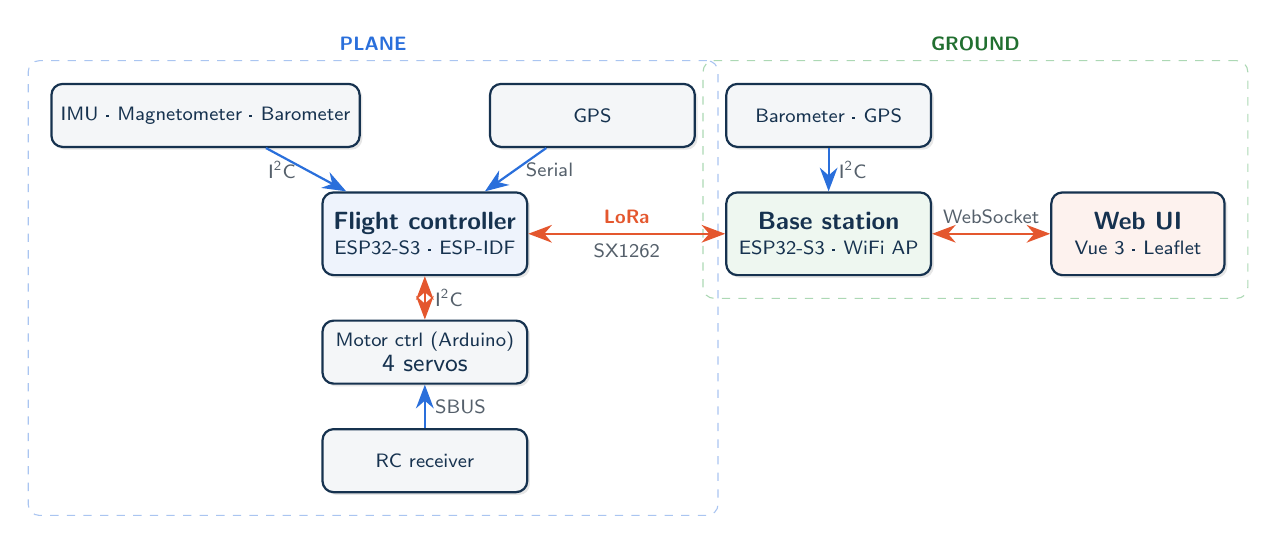
\begin{tikzpicture}[node distance=1.1cm and 1.6cm]
  % ---- Plane side ----
  \node[box, fill=skyblue!8] (fc) {\textbf{Flight controller}\\[-2pt]{\scriptsize ESP32-S3 · ESP-IDF}};
  \node[box, above left=0.55cm and -0.5cm of fc, minimum height=0.8cm] (imu)
    {\scriptsize IMU · Magnetometer · Barometer};
  \node[box, above right=0.55cm and -0.5cm of fc, minimum height=0.8cm] (gps)
    {\scriptsize GPS};
  \node[box, below=0.55cm of fc, minimum height=0.8cm] (mc)
    {\scriptsize Motor ctrl (Arduino)\\[-2pt]4 servos};
  \node[box, below=0.55cm of mc, minimum height=0.8cm] (rc)
    {\scriptsize RC receiver};

  % ---- Base side ----
  \node[box, right=2.5cm of fc, fill=leaf!8] (bs)
    {\textbf{Base station}\\[-2pt]{\scriptsize ESP32-S3 · WiFi AP}};
  \node[box, above=0.55cm of bs, minimum height=0.8cm] (bssens)
    {\scriptsize Barometer · GPS};
  \node[box, right=1.5cm of bs, fill=signal!8, minimum width=2.2cm] (web)
    {\textbf{Web UI}\\[-2pt]{\scriptsize Vue 3 · Leaflet}};

  % ---- Edges ----
  \draw[link] (imu) -- node[left, font=\scriptsize, text=slate]{I\textsuperscript{2}C} (fc);
  \draw[link] (gps) -- node[right, font=\scriptsize, text=slate]{Serial} (fc);
  \draw[link] (bssens) -- (bs) node[midway, right, font=\scriptsize, text=slate] {I\textsuperscript{2}C};;
  \draw[biln]  (fc) -- (mc) node[midway, right, font=\scriptsize, text=slate] {I\textsuperscript{2}C};
  \draw[link]  (rc) -- (mc) node[midway, right, font=\scriptsize, text=slate] {SBUS};
  \draw[biln]  (fc) -- node[above, font=\scriptsize\bfseries, text=signal]{LoRa}
                      node[below, font=\scriptsize, text=slate]{SX1262} (bs);
  \draw[biln]  (bs) -- node[above, font=\scriptsize, text=slate]{WebSocket} (web);

  % background groupings
  \begin{scope}[on background layer]
    \node[fit=(imu)(gps)(fc)(mc)(rc), draw=skyblue!40, dashed, rounded corners,
          inner sep=8pt, label={[skyblue, font=\scriptsize\bfseries]above:PLANE}] {};
    \node[fit=(bs)(bssens)(web), draw=leaf!40, dashed, rounded corners,
          inner sep=8pt, label={[leaf!70!black, font=\scriptsize\bfseries]above:GROUND}] {};
  \end{scope}
\end{tikzpicture}
\end{document}
